\chapter{Onderzoek}
\textit{In dit hoofdstuk worden de werkzaamheden met betrekking tot het uitvoeren van het onderzoek beschreven. De aanleiding voor het onderzoek is te vinden in hoofdstuk \ref{Aanpak}, waarin wordt beschreven waarom dit onderzoek meerwaarde heeft binnen de opdracht.}

Het onderzoek dient voor het opstellen van het adviesrapport waarin protocollen worden  gepresenteerd  aan Quintor die mogelijk geïmplementeerd kunnen worden tijdens de realisatie van het Proof-of-Concept. Het betreft exploratief onderzoek waarin case-study gebruikt wordt om een gedetailleerde omschrijving van de onderdelen Identity Management en Distributed Network op te stellen van Blockchain implementaties die geselecteerd zijn in hoofdstuk \ref{selectie}. De kennis die hiermee wordt opgebouwd kan eventueel gebruikt worden in vervolgonderzoek.

In het onderzoek staat de onderstaande hoofdvraag centraal:
\begin{formal}
  Welke protocol implementaties kunnen toegepast worden om de onderdelen Distributed Network en Identity Management te realiseren voor een Blockchain implementatie?
\end{formal}

Omdat de hoofdvraag te groot is om in een keer te beantwoorden is het opgesplitst in de volgende deelvragen:

\begin{enumerate}[noitemsep]
  \item "Welke soorten gedistribueerde netwerken worden er gebruikt?"
  \item "Hoe werken de gedistribueerde netwerken en tegen welke gevaren zijn ze bestendig?"
  \item "Hoe wordt er omgegaan met de identiteit van de gebruiker?
\end{enumerate}

Op de volgende pagina's is per deelvraag behandeld wat de bijdrage van het antwoord oplevert aan de doelstelling, hoe de vraag beantwoord is en wordt er concreet de bevindingen besproken.

\clearpage
\section{Opzet}

Om te achterhalen welke protocol implementaties toegepast kunnen worden om de onderdelen Distributed Network en Identity Management te realiseren voer ik kwalitatief, exploratief onderzoek uit. Door het uitgevoerde vooronderzoek heb ik wel basiskennis over de onderdelen, maar weet ik nog niet de details. Om die reden heb ik er dan ook voor gekozen om het exploratief aan te pakken. Het gevaar hierbij is dat er teveel informatie geanalyseerd wordt waardoor het onderzoek te uitgebreid wordt.

\subsection{Dataverzameling}

De benodigde data zal ik verzamelen door het uitvoeren van deskresearch, waarbij ik de geselecteerde Blockchain protocol implementaties zal analyseren. De data die ik hiervoor nodig hebt komt vooral uit de whitepapers die beschikbaar zijn voor elke implementatie. Daarnaast worden er zo veel mogelijk academische bronnen gebruikt. Om deze, mogelijk aanvullende, academische bronnen te vinden zal ik gebruik maken van het schoolportaal en Google Scholar. Hierbij zal er gelet worden op de kwaliteit van de studie, door te achterhalen of het gebruikt wordt in andere studies en te kijken of het peer reviewed is.

\subsection{Dataomschrijving}

De Blockchain implementaties zullen in eerste instantie geselecteerd worden op de aanwezigheid van het onderdeel Identity Management. Hierbij zal ik kijken of de implementatie actief iets onderneemt voor bijvoorbeeld het verhogen van de privacy van de gebruiker. Daarnaast zal er gekeken worden naar de beschikbare hoeveelheid informatie.

\subsection{Analysemethode}

De methode die ik zal gebruiken voor het analyseren van de data is het uitvoeren van cumulatieve case-studies. Hierbij zullen er meerdere bronnen bekeken worden van een Blockchain implementatie waarna een aggregatie gemaakt wordt van de benodigde data voor het beantwoorden van de opgestelde vragen.

\newpage
\section{Soorten netwerken}

\textit{In dit hoofdstuk wordt de vraag ``Welke soorten gedistribueerde netwerken worden er gebruikt?'' behandeld. Het doel van de vraag is om de architectuurkeuzes op het gebied van het Distributed Network onderdeel op te stellen, en waar mogelijk is de implicaties van de keuze tegenover het Identity Management onderdeel.}

% In het vooronderzoek is er gevonden dat het consensusproces van grote invloed kan zijn op de architectuurkeuzes van het gedistribueerd netwerk. Er is dan ook voor gekozen om in het onderzoek het netwerksoort synoniem te stellen aan het type consensus die de implementatie gebruikt.

\subsection{Aanpak}

\begin{wrapfigure}[14]{r}{0.5\textwidth}
  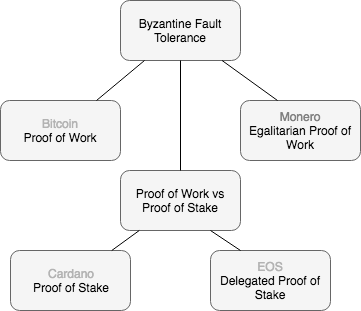
\includegraphics[width=0.5\textwidth]{figures/uitwerking_soorten}
  \caption[Opbouw beantwoording ``Soorten netwerken'']{Termen die als leidraad gebruikt zijn om het resultaat te beschrijven}
  \label{opbouw:netwerken}
\end{wrapfigure}

In fig. \ref{opbouw:netwerken} is te zien welke (globale) termen er gebruikt zijn om de benodigde informatie te vinden. In de meeste gevallen is de beschikbare whitepaper van de implementatie voldoende geweest om de werking van het consensus te beschrijven. Hieronder is de werkwijze en denkwijze uitgeschreven per individueel onderdeel.

\subsubsection{Byzantine Fault Tolerance}
Om deze vraag te beantwoorden is allereerst gezocht naar achtergrondinformatie over consensus en wat het doel ervan is. In het vooronderzoek is er informatie gevonden over het Byzantine Generals Problem \citep{lamport1982byzantine}, waarin, vertaald naar de IT-wereld, wordt gesteld dat het essentieel is voor een betrouwbaar computersysteem om te gaan met fouten in de componenten, waardoor het kan voorkomen dat er conflicterende informatie verstuurd wordt naar de andere componenten van het systeem. 

\subsubsection{Proof of Work}
Hierna zijn bij de implementaties de manier waarop consensus behaald wordt onderzocht. Voor het beschrijven van het Proof of Work algoritme is er gebruik gemaakt van de originele presentatie van het Bitcoin protocol door \cite{nakamoto2008bitcoin}, hierin was alle informatie te vinden die benodigd was. Het egalitarian Proof of Work zoals in gebruik bij Monero is beschreven in \cite{van2013cryptonote} waarin de verschillen en tekortkomingen van het Proof of Work zoals in gebruik bij Bitcoin uiteengezet wordt.

\newpage
\subsubsection{Proof of Stake}
Om een indicatie te geven van de grootste tekortkomingen op het gebied van Proof of Work en redenenen waarom Blockchain implementaties kiezen voor het implementeren van Proof of Stake is er gebruik gemaakt van de whitepaper van Cardano \cite{kiayias2017ouroboros}, waarin de gemotiveerd wordt waarom er voor Proof of Stake is gekozen in plaats van Proof of Work. Naar aanleiding van de primaire reden, namelijk dat Proof of Work enorm veel stroom verspilt, is er gezocht naar een studie die deze claim kan bevestigen, waarbij de studie van \cite{ODwyer:Bitcoin} gebruikt is om dit te bevestigen.

Bij het beschrijven van Delegated Proof of Stake zoals in gebruik bij EOS, bleek de whitepaper niet voldoende informatie te bevatten om het functioneel te beschrijven. Hiervoor is er dan ook een artikel gebruikt dat geschreven is door \cite{steemit:eos_dpos}, waarin het algoritme uitgelegd wordt.

\subsection{Conclusie}

Een gedistribueerd netwerk binnen Blockchain is getypeerd aan het consensus protocol dat gebruikt wordt. In het onderzoek zijn er twee primaire soorten geïdentificeerd, netwerken die gebruik maken van Proof of Stake of van Proof of Work, waarbij Proof of Work gebruik maakt van de rekenkracht van een \gls{node} en Proof of Stake gebruik maakt van de \gls{stake} van een \gls{node}.

\newpage
\section{Functionaliteit en gevaren}

\textit{In dit hoofdstuk wordt de vraag ``Hoe werken de gedistribueerde netwerken en tegen welke gevaren zijn ze bestendig?'' behandeld. Het doel van de vraag is om de werking van het gedistribueerd netwerk in kaart te brengen en tegenmaatregelen tegen aanvallen die in de functionaliteit verwerkt zitten te beschrijven.}

Deze vraag is opgesteld naar aanleiding van de criteria ``het moet resistant zijn tegen aanvallen'' die gesteld is in de opdrachtformulering zoals gegeven door Quintor, in te zien in bijlage \ref{appendix:opdrachtformulering}. Het eerste idee om deze vraag te beantwoorden was om een vergelijking te maken tussen de implementaties op het gebied van veiligheid, waarbij er onderzocht zou worden of een aanval op de implementatie uitgevoerd was. Dit zou uiteindelijk een ``beste'' implementatie opleveren die geadviseerd zou worden in het adviesrapport. Uiteindelijk is dit idee niet gebruikt omdat er een aantal redenenen zijn waarom dit niet zou werken:

\begin{itemize}
  \item \textbf{Protocol volwassenheid}
  \\ Het Bitcoin protocol bestaat al sinds 2011, terwijl het Monero protocol sinds 2014 bestaat. In het begin heeft Bitcoin waarschijnlijk veel te verduren gehad qua aanvallen, waardoor het via bovenstaande vergelijking slecht uit zou komen. Daarentegen heeft Monero gedurende de drie jaar zowel verbeteringen als lessen getrokken uit het Bitcoin protocol.

  \item \textbf{Adoptie van de technologie}
  \\ Proof of Work implementaties zijn vatbaar voor een \gls{majority_attack}, waarbij een gebruiker 51\% van de rekenkracht binnen het netwerk in handen moeten hebben om transacties in de Blockchain te registreren zonder dat er validatie te pas komt. Hoe minder gebruikers, hoe minder de benodigde rekenkracht om dit uit te voeren.
\end{itemize}

Om deze reden is er besloten om met de Blockchain expert over de aanpak en uiteindelijke doel van deze vraag te discussiëren, wat ertoe heeft geleid dat de focus van de vraag veranderd is van een vergelijking doen op basis van de veiligheid, het een meer beschrijvende vorm heeft gekregen waar er gekeken wordt naar componenten van het netwerk: discovery protocol, hoe informatie verstuurd wordt tussen twee \glspl{node} en wanneer mogelijk de knelpunten met betrekking tot aanvallen binnen deze componenten.

\newpage
\subsection{Aanpak}

\begin{wrapfigure}[14]{r}{0.6\textwidth}
  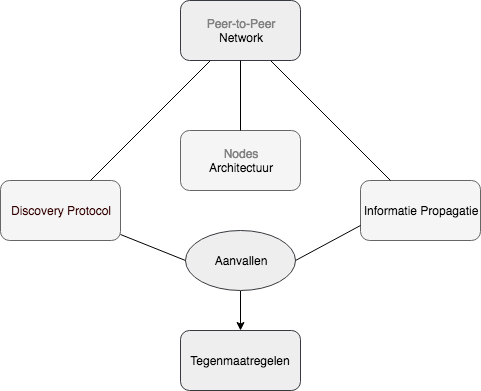
\includegraphics[width=0.6\textwidth]{figures/uitwerking_functionaliteit}
  \caption[Opbouw beantwoording ``Functionaliteit en gevaren'']{Componenten en termen die als leidraad gebruikt zijn om het resultaat te beschrijven.}
  \label{opbouw:functionaliteit}
\end{wrapfigure}

In fig. \ref{opbouw:netwerken} is te zien welke componenten er gebruikt zijn om de benodigde informatie te vinden. Hieronder is de werkwijze en denkwijze uitgeschreven per individueel onderdeel.

\subsubsection{Aanvallen}

Allereerst is er begonnen met het zoeken naar de verschillende aanvallen die mogelijk zijn op Blockchain implementaties. Binnen het gesprek met de Blockchain Expert is hierbij het woord threat model gevallen, en zijn er een aantal aanvallen aan bod gekomen:

\begin{itemize}
  \item \textbf{Eclipse attack}
  \\ Meer informatie en de definitie van een eclipse attack is gevonden in de studie van \cite{heilman2015eclipse}.

  \item \textbf{Majority attack}
  \\ De majority attack staat beschreven op de wiki van Bitcoin, waarbij er uitgelegd wordt wat het is, wat er mee mogelijk is en waarom het bijna niet uit te voeren is.

  \item \textbf{Denial of Service}
  \\ Bij Denial of Service gaat het om meerdere manieren om de uitvoering van processen binnen het netwerk te verstoren, waardoor er niet een specifieke bron te vinden is voor alle mogelijke aanvallen.

  \item \textbf{Sybil attack}
  \\ Voor het beschrijven van de sybil attack in relatie tot Blockchain is er gebruik gemaakt van de studie gedaan door \cite{conti2017survey}.

  \item \textbf{Double spending}
  \\ Informatie double spending is gevonden in de studie van \cite{karame2012double}.
\end{itemize}

Een van de knelpunten bij het beschrijven van een aanval was een studie vinden die aantoonde wat het gevolg ervan was binnen een Blockchain implementatie.

\subsubsection{Network}

Voor het beschrijven van de verschillende netwerken is er gebruikt gemaakt van niet wetenschappelijke bronnen zoals wiki's of blogs. De reden hiervoor is dat een whitepaper van een Blockchain implementatie zelden de architectuur van het netwerk beschrijft. Deze informatie is dan ook gebruikt om de verschillende componenten van het netwerk te beschrijven.

\subsection{Conclusie}

\paragraph{Bitoin} Het netwerk van Bitcoin communiceert via TCP/IP en maakt gebruik van bootstrap nodes waarmee connectie wordt gemaakt op het moment dat een nieuwe deelnemer het netwerk wilt toetreden. Informatie wordt verstuurd door een voorafgedefinieerde set aan berichttypes: \textit{inv}, \textit{tx}, \textit{block}, \textit{getdata}, waarbij een \textit{inv} bericht gebruikt wordt ter inventarisatie over de beschikbaarheid van data, \textit{tx} bericht om een transactie te versturen, \textit{block} bericht om een block te versturen, \textit{getdata} bericht om data op te vragen. \\ \\ Op het Bitcoin netwerk zijn meerdere aanvallen in de loop der jaren uitgevoerd en geïdentificeerd, een studie uit 2015 gedaan door \cite{heilman2015eclipse} toont aan dat het Peer Discovery mechanisme vatbaar is voor een Sybil Attack. \cite{nakamoto2008bitcoin} stelt dat de voordelen van het uitvoeren van een majority attack niet opweegt tegen de kosten voor de benodigde hardware om de rekenkracht te behalen. \cite{eyal2014majority} beschrijft dat het niet nodig is om een merendeel van de rekenkracht te bezitten en introduceert de aanval \gls{selfish_mining}.

\newpage
\paragraph{Cardano} Het netwerk van Cardano communiceert via TCP/IP en maakt gebruik van het Kademlia protocol waardoor het maar nodig is om één bootstrap node te gebruiken om het netwerk toe te treden. De achterliggende structuur van Kademlia is een Binary Tree waarbij de positie van een deelnemer in de Binary Tree bepaald wordt door een unieke prefix van de identificatiecode. Het protocol garandeert dat een deelnemer in verbinding staat met ten minste één andere deelnemer. Informatie wordt uitgewisseld door drie abstracte berichttypes: \textit{inv}, \textit{req}, en \textit{data}. Het \textit{inv} bericht wordt gebruikt om aan te geven dat er data beschikbaar is, het \textit{req} bericht wordt gebruikt om beschikbare data op te vragen en het \textit{data} bericht wordt vervolgens gebruikt om de data te versturen. \\ \\ Implementaties die gebruik maken van \acrshort{PoS} zijn afhankelijk van de manier waarop een leiderschapsverkiezing wordt gesimuleerd, waarbij er grote kans is dat het gevoelig is voor beïnvloedingen van kwaadwillende deelnemers in het netwerk in de vorm van een Sybil Attack. Cardano heeft een zwak punt in het Kademlia netwerk geïdentificeerd waardoor het mogelijk zou zijn om Eclipse Attack uit te voeren.

\paragraph{Monero} Het netwerk van Monero maakt gebruik van het \acrfull{I2P} protocol, dat zowel UDP/IP als TCP/IP ondersteund. Om het netwerk toe te treden wordt er gebruik gemaakt van bootstrap nodes die vastgelegd zijn in de broncode. Communicatie wordt gedaan door middel van \Glspl{tunnel}, waarbij elke deelnemer twee \Glspl{tunnel}, een inkomende en een uitgaande, heeft voor elke connectie.

\paragraph{EOS} \textit{Ten tijde van het onderzoek is er geen technische beschrijving beschikbaar over het netwerk component van EOS.}






\newpage
\section{Identiteit}

\textit{In dit hoofdstuk wordt de vraag ``Hoe wordt er omgegaan met de identiteit van de gebruiker binnen de implementatie?'' behandeld. Het doel van de vraag is om de mogelijkheden en toepassingen van identiteit te beschrijven aan de hand van de geselecteerde implementaties.}

\begin{figure}[h]
  \centering
  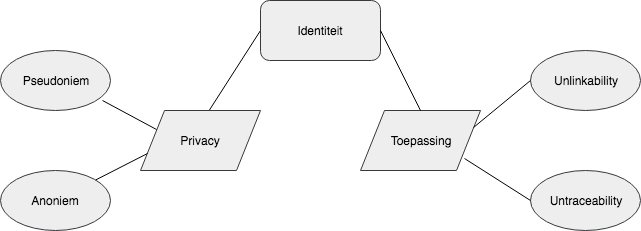
\includegraphics[width=0.8\textwidth]{figures/uitwerking_identity}
  \caption[Opbouw beantwoording ``Identiteit'']{Termen die als leidraad gebruikt zijn om het resultaat te beschrijven}
  \label{opbouw:identiteit}
\end{figure}

\subsection{Aanpak}

In fig. \ref{opbouw:identiteit} is te zien welke componenten er gebruikt zijn om de benodigde informatie te vinden. In het vooronderzoek is er gevonden dat identiteit eigenlijk uit twee onderdelen bestaat binnen Blockchain implementaties. Het privacy gedeelte, wat bepaalt of de identiteit zoals in gebruik bij de implementatie pseudoniem of anoniem is. Daarnaast is de toepassing van de identiteit van belang. Een voorbeeld van de toepassing van de identiteit is bijvoorbeeld het ondertekenen van transacties. 

\subsubsection{Identiteit}

In het vooronderzoek is er ook vastgesteld dat de identiteit van een gebruiker en hoe het gebruikt wordt is terug te leiden naar de architectuur van de Blockchain. De kern van Blockchain implementaties met betrekking tot identiteit en de toepassing daarvan is het gebruik van public- en private key cryptografie. Bij dit onderdeel was het belangrijk om niet teveel te beschrijven van de onderliggende cryptografie, omdat dit buiten de scope van de vraag valt. 

\newpage
\subsection{Conclusie}

\paragraph{Bitcoin} is een public Blockchain waarbij de gehele historie van transacties publiekelijk in te zien is. Een deelnemer in het Bitcoin netwerk wordt geïdentificeerd aan de hand van zijn public key. Deze public key wordt onder andere opgenomen in transacties om de betaler en de ontvanger te registreren. In een studie gedaan door \cite{reid2013analysis} wordt er een analyse model opgezet dat aantoont dat het Bitcoin protocol niet aan de untraceability eis voldoet.

\paragraph{Cardano} is een public Blockchain waarbij de gehele historie van transacties publiekelijk in te zien is. Cardano maakt gebruik van public- en private key cryptografie om pseudonimiteit te waarborgen. Deze keys worden gebruikt om een transactie van een bestemming te voorzien, waarbij er drie definities van adressen gebruikt worden: een public key address, een script address en een redeem address.

\paragraph{EOS} is een consortium Blockchain waarbij gebruikers zichzelf identificeren met een unieke naam van maximaal twaalf karakters. Om te participeren binnen het netwerk dient er toegang verleent te worden door een authenticatie proces alvorens de deelnemer wordt toegelaten.  Handeling binnen het netwerk worden gevalideerd door een Role Based Permissie systeem, waarbij permissies gekoppeld zijn aan actions die vastgelegd zijn in de lokale database.

\paragraph{Monero} is een public Blockchain waarbij de gehele historie van transacties publiekelijk in te zien is. Binnen Monero heeft elke deelnemer een account die gebaseerd is op twee keys: Spend Key en een View Key. Door het afleiden van een eenmalige public key, ook wel een Stealth Address genoemd, uit de Spend Key en View Key garandeert het Monero protocol unlinkability. Untraceability wordt behaald door het gebruik van Ring Signatures. Hierbij worden meerdere Stealth Addresses toegevoegd aan een transactie, waarbij een afkomstig van de verstuurder van de transactie en de rest aangevuld door eerder gebruikte Stealth Addresses in de Blockchain. Hierdoor wordt de herkomst van een transactie gemaskeerd. 

\newpage
\section{Conclusie}

In het onderzoek is er een selectie van Blockchain implementaties onderzocht op de onderdelen Identity Management en Distributed Network. Door het uitvoeren van exploratief onderzoek waarin case-study gebruikt is om een gedetailleerde omschrijving van desbetreffende onderdelen op te stellen. De hoofdvraag \textit{Welke protocol implementaties kunnen toegepast worden om de onderdelen Distributed Network en Identity Management te realiseren voor een Blockchain implementatie?} is opgedeeld in deelvragen:

\begin{enumerate}[noitemsep]
  \item "Welke soorten gedistribueerde netwerken worden er gebruikt?"
  \item "Hoe werken de gedistribueerde netwerken en tegen welke gevaren zijn ze bestendig?"
  \item "Hoe wordt er omgegaan met de identiteit van de gebruiker?
\end{enumerate}

Uit de resultaten van de deelvragen is uiteindelijk een antwoord op de hoofdvraag gekomen. Voor het onderdeel Distributed Network kan er gebruik gemaakt worden van:

\paragraph{Kademlia}

Een bestaand protocol gerealiseerd door \cite{maymounkov2002kademlia}. Dit protocol heeft een aantal wijzigingen binnen Cardano, zoals het versturen van informatie gaat over TCP/IP en er is een uitbreiding gemaakt op de manier waarop identificatiecodes toegekend worden aan deelnemers om een mogelijke Sybil Attack uit te sluiten.

\paragraph{Bitcoin}

Communicatie binnen het Bitcoin netwerk verloopt over TCP/IP waarbij informatie wordt verstuurd door inv, tx, block en getdata berichten. Het maakt gebruik van Proof of Work om consensus te bereiken over de staat van de Blockchain.

\paragraph{Monero}

De Monero implementatie is gefocust op het bevorderen van de privacy binnen Blockchain implementaties. Voor het netwerk is dat dan ook niet anders. Het maakt gebruik van The Invisible Project om anonimiteit in het netwerk te waarborgen.

Voor het onderdeel Identity Management is het mogelijk om de volgende protocollen toe te passen:

\paragraph{Bitcoin} het Bitcoin protocol maakt gebruik van het UTXO-model, waarin public- en private keys gebruikt worden om de betaler en ontvanger te registreren binnen een transactie. Door het gebruik van het analysemodel gepresenteerd door \cite{reid2013analysis} is aangetoond dat Bitcoin niet aan de untraceability en unlinkability eis voldoet.

\paragraph{EOS} maakt gebruik van een account-model, waarin een gebruiker een unieke naam van maximaal twaalf karakters hanteert als identiteit. Daarnaast hanteert EOS een Role Based Permission Management systeem, waarbij het mogelijk is actions en handlers te definiëren.



